\documentclass{standalone}
%% Show/hide steps for standalone work — edit this line:
\makeatletter\AtBeginDocument{\@buildstepset{1,2,3,4,5,6,7,8,9,10}}\makeatother
\usepackage{tikz}
\usetikzlibrary{intersections,calc}
\usepackage{amsmath}
\usepackage{hsbcommon}
\begin{document}
    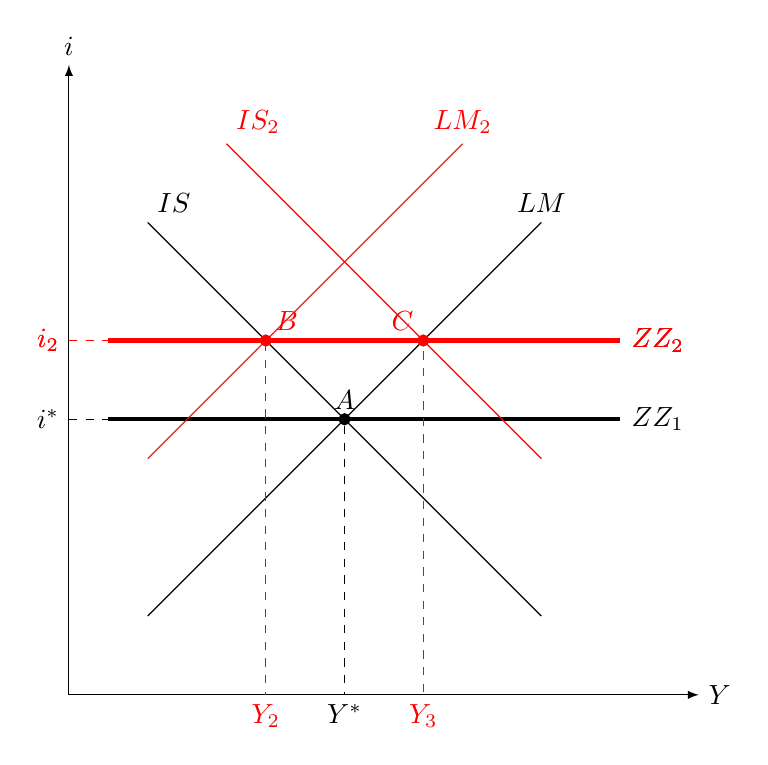
\begin{tikzpicture}
        \draw[->,>=latex] (0,0) -- (8,0) node (Y) [right] {$Y$};
        \draw[->,>=latex] (0,0) -- (0,8) node (i) [above] {$i$};

        \draw[name path=is] (1,6) node[above right] {$IS$} -- (6,1);
        \draw[name path=lm] (1,1) -- (6,6) node[above] {$LM$};

        \path [name intersections={of=is and lm, by=E}];
        \filldraw (E) circle (2pt) node[above] {$A$};
        \draw[dashed] (i |- E) node [left] {$i^*$} -- (E) -- (E |- Y) node [below] {$Y^*$};

        %% ZZ1 curve at equilibrium height
        \draw[ultra thick, name path=zz] (0.5, |- E) -- (7, |- E) node [right] {$ZZ_1$};

        %% Step 1: ZZ shifts up → B (IS∩ZZ2) and C (LM∩ZZ2)
        \ifstep{1}{
            \begin{scope}[color=red, yshift=1cm]
                \draw[ultra thick, name path=zz2] (0.5,3.5) -- (7,3.5) node [right] {$ZZ_2$};
                \path [name intersections={of=is and zz2, by=F}];
                \path [name intersections={of=lm and zz2, by=G}];
            \end{scope}
        }

        %% Step 2: LM shifts up to pass through C → new equilibrium at Y_2
        \ifstep{2}{
            \begin{scope}[color=red, yshift=1cm]
                \draw[ultra thick, name path=zz2] (0.5,3.5) -- (7,3.5) node [right] {$ZZ_2$};
                \filldraw (F) circle (2pt) node[above right] {$B$};
                \path [name intersections={of=is and zz2, by=F}];
                \path [name intersections={of=lm and zz2, by=G}];
                \draw[name path=lm2] (1,2) -- (5,6) node[above] {$LM_2$};
                \draw[dashed] (i |- F) node [left] {$i_2$} -- (F) -- (F |- Y) node [below] {$Y_2$};
            \end{scope}
        }

        %% Step 3: IS shifts → new equilibrium at Y_3
        \ifstep{3}{
            \begin{scope}[color=red, yshift=1cm]
                \draw[ultra thick, name path=zz2] (0.5,3.5) -- (7,3.5) node [right] {$ZZ_2$};
                \filldraw (G) circle (2pt) node[above left]  {$C$};
                \path [name intersections={of=lm and zz2, by=G}];
                \draw[name path=is2] (2,6) node[above right] {$IS_2$} -- (6,2);
                \draw[dashed] (i |- G) node [left] {$i_2$} -- (G) -- (G |- Y) node [below] {$Y_3$};
            \end{scope}
        }

    \end{tikzpicture}
\end{document}